\documentclass[a4paper,12pt]{article}
\usepackage[a4paper,top=1.3cm,bottom=2cm,left=1.5cm,right=1.5cm,marginparwidth=0.75cm]{geometry}
\usepackage{setspace}
\usepackage{cmap}
\usepackage{mathtext}
\usepackage[T2A]{fontenc}
\usepackage[utf8]{inputenc}
\usepackage[english,russian]{babel}
\usepackage{multirow}
\usepackage{graphicx}
\usepackage{wrapfig}
\usepackage{tabularx}
\usepackage{float}
\usepackage{longtable}
\usepackage{hyperref}
\hypersetup{colorlinks=true,urlcolor=blue}
\usepackage[rgb]{xcolor}
\usepackage{amsmath,amsfonts,amssymb,amsthm}
\usepackage{icomma}
% $\mathtoolsset{showonlyrefs=false}$
\usepackage{euscript}
\usepackage{mathrsfs}
\usepackage{float}
\usepackage{amsmath}
\setlength{\parindent}{1cm} % Устанавливает отступ в 1.5 см для всех абзацев


\DeclareMathOperator{\sgn}{\mathop{sgn}}
\newcommand*{\hm}[1]{#1\nobreak\discretionary{}
	{\hbox{$\mathsurround=0pt #1$}}{}}

\title{\textbf{Отчёт о выполненой лабораторной работе \\ \textit{Эффект Джоуля–Томсона (2.1.6)}}}

\author{Каплин Артём Б01-402}
\date{24 марта 2025}


\begin{document}

\maketitle
	
	\section{Введение}
	
	\textbf{Цель работы:} : 1) определить изменения температуры углекислого газа при протекании через малопроницаемую перегородку при разных начальных значениях температуры, вычислить коэффициент Джоуля-Томсона; 2) вычислить по результатам опытов коэффициенты $a$ и $b$ модели Вандер-Ваальса, а также температуру инверсии $T_{\text{инв}}$.\\
    \\
    \textbf{Оборудование:} трубка с пористой перегородкой; труба Дьюара; термостат
    жидкостной; термопара; вольтметр универсальный цифрововй; баллон с углекислым газом; манометр.
	
	\section{Теоретические сведения }
    
Эффектом Джоуля–Томсона называется изменение температуры газа при его адиабатическом дросселировании. Процесс дросселирования — это медленное протекание газа через дроссель под воздействием перепада давления. Дросселем можно назвать препятствие потоку газа в трубе в виде, например, пористой перегородки. Почти полностью закрытый и слегка пропускающий газ кран также можно считать дросселем. Пористой перегородкой может служить диск из керамики или пористого стекла. При дросселировании температура газа может как увеличиваться, так и уменьшаться. Очевидно, что такой процесс необратим. Рассмотрим его подробнее.\\
 
Получим теоретическое выражения для расчёта величины эффекта Джоуля–Томсона.

\begin{figure}[h!]
        \centering
        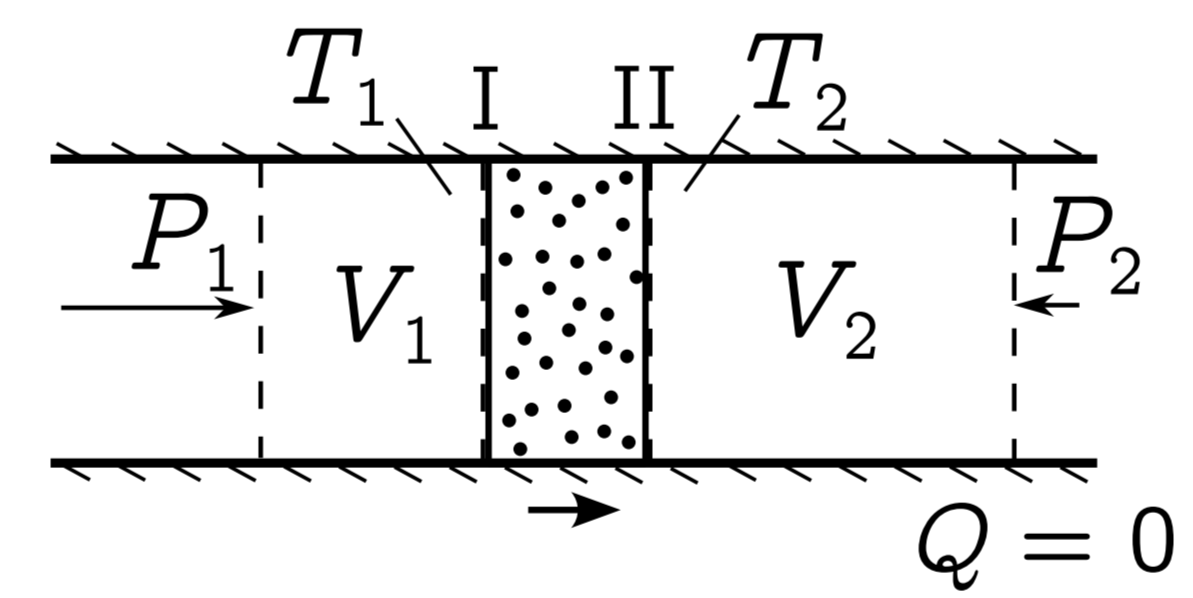
\includegraphics[scale=0.2]{216.png}
        \caption{
         Принципиальная схема эффекта Джоуля–Томсона
        }
 \end{figure} 




На рис. (1) изображена адиабатически изолированная труба с пористой перегородкой. Заметим, что разность давлений всегда $P_2 - P_1 = \Delta P < 0$, что говорит о существенной необратимости этого процесса. В силу его адиабатичности можно записать очевидное равенство:

\begin{equation}
Q = 0 = U_2 - U_1 + P_2V_2 - P_1V_1
\end{equation}

Здесь работа внешних сил равна $P_1V_1 < 0$, а $P_2V_2$ — работа самого газа, она положительна. Отсюда следует, что:

\begin{equation}
U_1 + P_1V_1 = U_2 + P_2V_2, \quad \text{т.е.} \quad I_1 = I_2.
\end{equation}

Значит, процесс дросселирования происходит при постоянстве энтальпии. 

В качестве характеристики процесса дросселирования введем величину, называемую коэффициентом Джоуля–Томсона:

\begin{equation}
\mu = \frac{\Delta T}{\Delta P},
\end{equation}

которая определяет эффект Джоуля–Томсона количественно. Поскольку для идеального газа энтальпия — однозначная функция температуры, то в связи с постоянством энтальпии для идеального газа $\Delta T = 0$, т.е. и $\mu = 0$. Конечно, для реального газа это уже далеко не так.

Рассмотрим так называемый дифференциальный эффект Джоуля–Томсона, т.е. эффект при малом перепаде давления на дросселе.

\begin{equation}
\mu = \left( \frac{\Delta T}{\Delta P} \right)_I \approx \left( \frac{\partial T}{\partial P} \right)_I.
\end{equation}

Запишем дифференциал энтальпии как функцию $T$ и $P$:

\begin{equation}
dI(T, P) = \left( \frac{\partial I}{\partial T} \right)_P dT + \left( \frac{\partial I}{\partial P} \right)_T dP = 0.
\end{equation}

Отсюда частная производная:

\begin{equation}
\left( \frac{\partial T}{\partial P} \right)_I = \mu = -\frac{\left( \frac{\partial I}{\partial P} \right)_T}{\left( \frac{\partial I}{\partial T} \right)_P} = -\frac{1}{C_P} \left( \frac{\partial I}{\partial P} \right)_T.
\end{equation}

Известна каноническая зависимость энтальпии от температуры и энтропии:

\begin{equation}
dI = T dS + V dP,
\end{equation}

Откуда при постоянной температуре искомая частная производная $\left( \frac{\partial I}{\partial P} \right)_T$ равна:

\begin{equation}
\left( \frac{\partial I}{\partial P} \right)_T = T \left( \frac{\partial S}{\partial P} \right)_T + V = -T \left( \frac{\partial V}{\partial T} \right)_P + V.
\end{equation}

Подставляя ее в (6), получим общее выражение для коэффициента Джоуля–Томсона при малом перепаде давления:

\begin{equation}
\mu \approx \left( \frac{\partial T}{\partial P} \right)_I = \frac{T \left( \frac{\partial V}{\partial T} \right)_P - V}{C_P}.
\end{equation}

Теперь из общего выражения (9) найдем коэффициент Джоуля–Томсона для газа Ван-дер-Ваальса. Для этого надо продифференцировать уравнение Ван-дер-Ваальса (  ) по температуре, считая давление $P$ постоянным:

\begin{equation}
-\frac{2a}{V^3} \left( \frac{\partial V}{\partial T} \right)_P (V - b) + \left( P + \frac{a}{V^2} \right) \left( \frac{\partial V}{\partial T} \right)_P = R.
\end{equation}

Искомая частная производная равна:

\begin{equation}
\left( \frac{\partial V}{\partial T} \right)_P = \frac{R}{P + \frac{a}{V^2} - \frac{2a(V - b)}{V^3}} = \frac{R(V - b)}{RT - \frac{2a(V - b)^2}{V^3}}.
\end{equation}

Для начала будем считать газ не очень плотным. Кроме того, пренебрежем величинами второго порядка относительно поправок $b$ и $a$. Тогда:

\begin{equation}
T \left( \frac{\partial V}{\partial T} \right)_P \approx \frac{V - b}{1 - \frac{2a}{RTV}} \approx (V - b) \left( 1 + \frac{2a}{RTV} \right) \approx V + \frac{2a}{RT} - b.
\end{equation}

Если подставить(9) в формулу для эффекта Джоуля–Томсона (12), получим окончательно:

\begin{equation}
\mu = \frac{\Delta T}{\Delta P} = \frac{\frac{2a}{RT} - b}{C_P}.
\end{equation}

Из этого выражения для $\mu$ сразу видно, что изменение температуры газа Ван-дер-Ваальса при необратимом расширении определяется поправками $a$ и $b$. При $a = b = 0$ $\mu = 0$. Кроме того, поправки $a$ и $b$ по-разному влияют на знак эффекта. Если силы взаимодействия между молекулами велики и преобладает поправка на давление, то можно считать $b = 0$, и тогда $\mu > 0$, т.е. $\Delta T < 0$ (газ охлаждается). Если силы взаимодействий малы и $a \to 0$, то преобладает поправка на объем $b$. В этом случае $\mu < 0$, и газ нагревается, т.е. $\Delta T > 0$ ($\Delta P < 0$).




\section{Экспериментальная установка}
Схема установки для исследования эффекта Джоуля–Томсона в углекислом газе
представлена на рис. 2. Основным элементом установки является трубка 1 с пористой
перегородкой 2, через которую пропускается двуокись углерода $CO_2$. Углекислый газ под повышенным давлением поступает в трубку через змеевик 5
из балластного баллона 6. Медный змеевик омывается водой и нагревает медленно
протекающий через него газ до температуры воды в термостате. Температура воды
измеряется встроенным в термостат термометром. Давление газа в трубке измеряется манометром М и регулируется вентилем В . Манометр М измеряет разность между давлением внутри трубки и наружным (атмосферным) давлением. Разность температур газа до и после перегородки измеряется термопарой медь–константан.
\begin{figure}[h!]
        \centering
        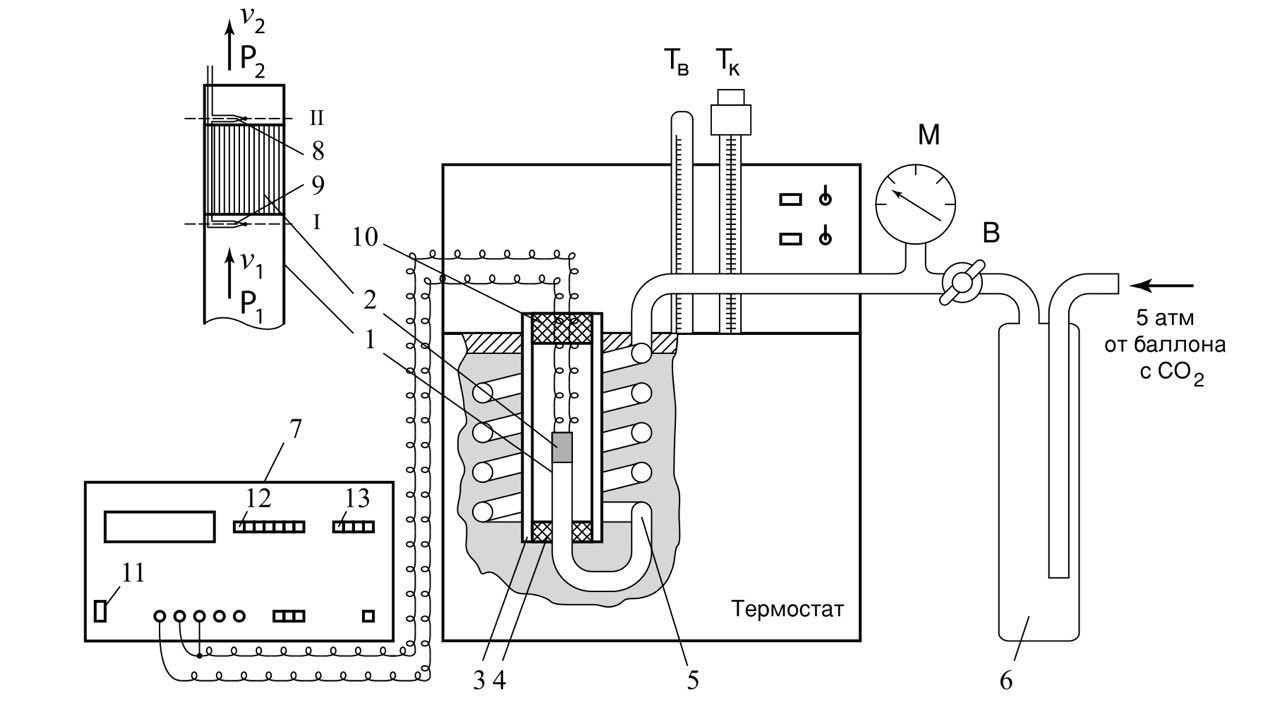
\includegraphics[scale=0.3]{ustj.jpg}
        \caption{
        Рис. 2. Экспериментальная установка
        }
 \end{figure} 



\section{Приборы и данные}
\begin{itemize}
    \item Цифровой мультиметр B7-78/1, погрешность измерения погрешность измерения постоянного напряжения 0,0035\% + 0,0005\% диапазона. 
    \item Манометр WIKA EN 837-1, класс точности 1,0.
    \item Термостат жидкостный ТЖ-ТС-01,  погрешность установления заданной температуры не более $0,02 ^\circ C$, погрешность поддержания температуры не более $0,01 ^\circ C$.

\end{itemize}

\section{Ход работы}

\begin{enumerate}
        \item Убедимся, что термостат залит водой, все электрические приборы
        заземлены.
        \item Включим термостат.
        \item Включим вольтметр . Начальные показания приборов $t_0 = 13,9 ^\circ C; \varepsilon_0 = -0,002 \text{мВ},$

где $t_0$ - начальная температура термостата с водой, $\varepsilon_0$ - показания вольтметра

        \item Проведем измерения при температурах $T_1 = 15$ \textdegree C,
        $T_2 = 33$ \textdegree C, $T_3 = 45$ \textdegree C, $T_4 = 57$ \textdegree C. Полученные данные представлены в приложении.

        \item Построим график зависимости разности темпераиур от перепада давления по МНК для четырёх температур.

        \begin{figure}[h!]
        \centering{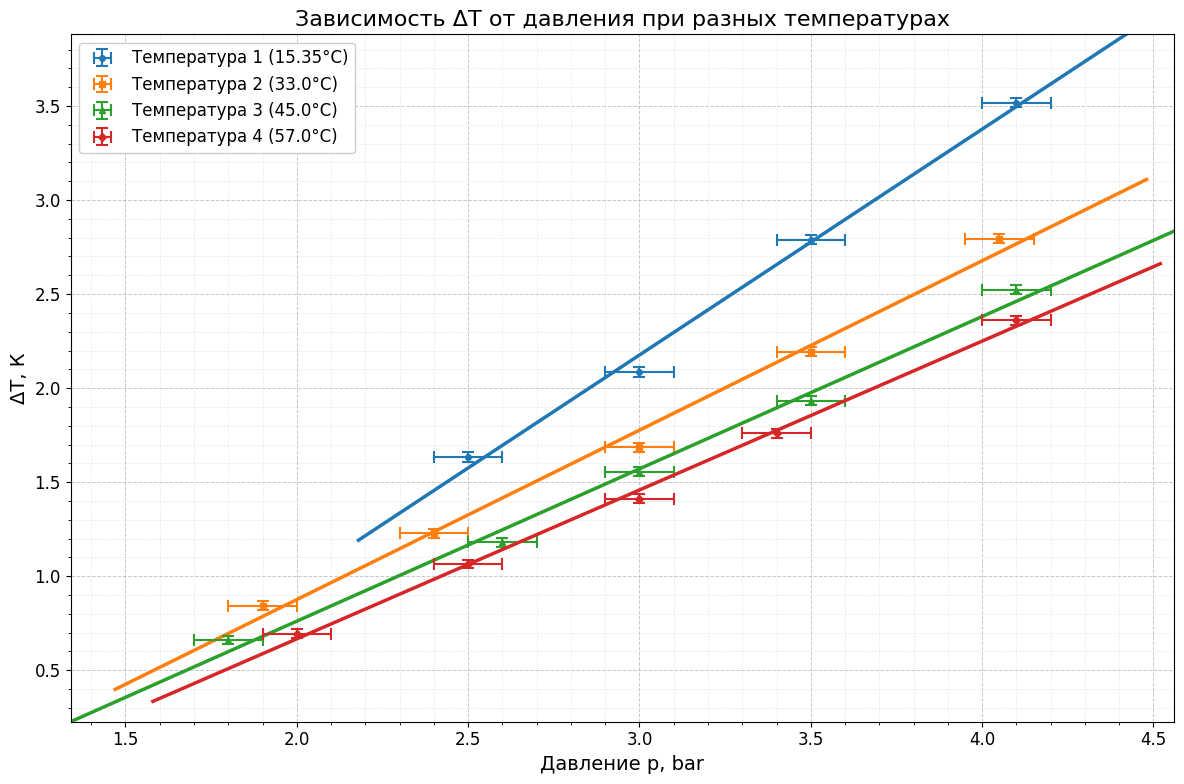
\includegraphics[width=1\textwidth]{gr1.png}}
        \caption[]{\label{} График №1 Зависимость разности температур от перепада давления $\Delta T(\Delta P)$}
        \end{figure}

        \item По наклону прямых получим значения коэффициентов Джоуля-Томсона для разных температур воды в термостате. 
\begin{table}[h!]
    \centering
    \begin{tabular}{|c|c|c|c|}
        \hline
        № & $\mu, \frac{\text{К}}{\text{бар}}$ & $\sigma_{\mu}, \frac{\text{К}}{\text{бар}}$ & $\varepsilon, \%$ \\
        \hline
        1 & $1.201$ & $0.046$ & $3.87$ \\
        \hline
        2 & $0.901$ & $0.035$ & $3.88$ \\
        \hline
        3 & $0.810$ & $0.030$ & $3.75$ \\
        \hline
	  4 & 0.792	&0.018&	2.24 \\
	  \hline
    \end{tabular}
    \caption{Таблица 5. Коэффициенты Джоуля-Томсона}
\end{table}

    \item По полученным коэфициентам Джоуля-Томсона постром график зависимости.

    \begin{figure}[h!]
\centering{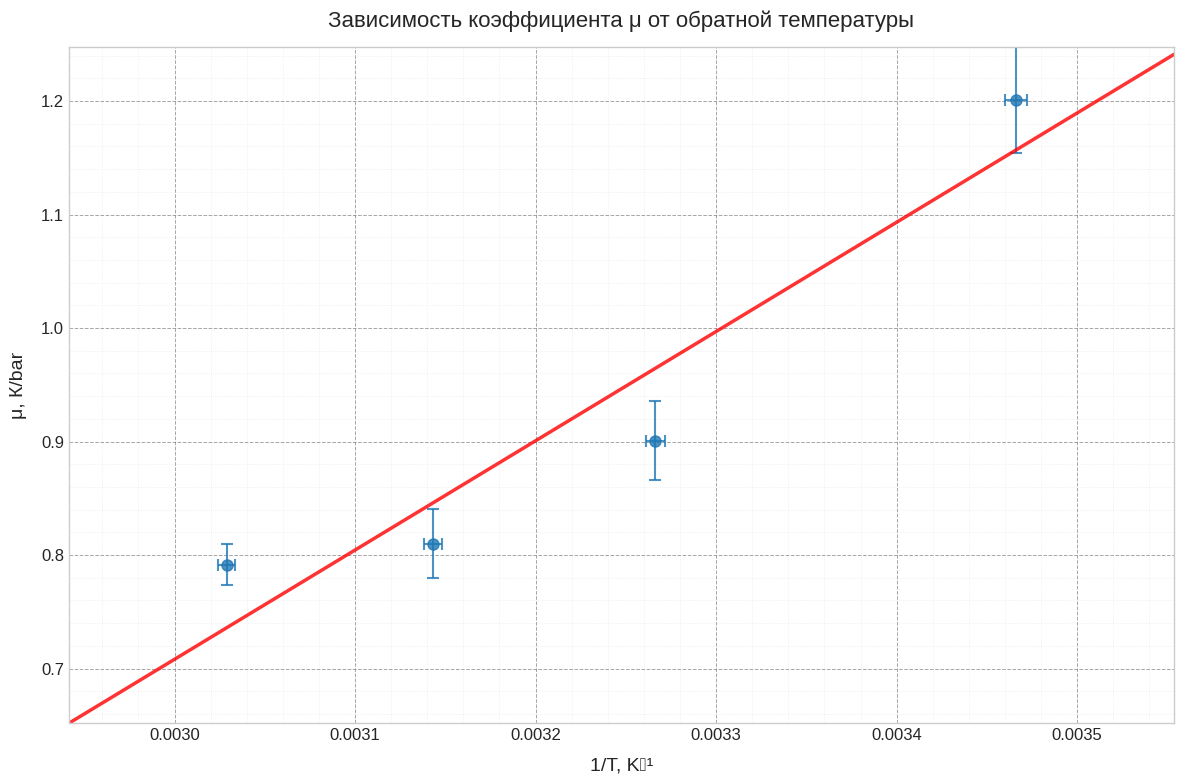
\includegraphics[width=1\textwidth]{gr2.png}}
\caption[]{\label{} График 2. Зависимости коэффициента Джоуля-Томсона от обратной температуры}
\end{figure}
    \item \[k = (963 \pm 157) \ \frac{K^2}{\text{бар}} \ \ \varepsilon_k = 16,3 \% \ \ \ \ \ b = \mu_0 = (-2.180 \pm 0.508) \ \frac{K}{\text{бар}} \ \ \varepsilon_{\mu_0} = 23 \% \]

    \item Найдем коэффициенты $a$ и $b$ для соответствующих температур попарно по формулам:
    \[a = \frac{kRC_p}{2} \ \ \ \ \ \ \ \ \ \ \\  b= \mu_0 C_p,\] где $C_p = 37,1 \frac{\text{Дж}}{\text{моль \ К}}$ табличное значение, взятое с книги Лабораторный практикум.
    
    \[a  = (1,484 \pm 0,242) \  \frac{H\cdot\text{ м} ^4}{\text{моль} ^2}  \ \ \ \ \ \ \varepsilon_a = 16,3 \%\ \ \ \ \ \ \ \ b = (8,09 \pm 1,86) \cdot 10^{-4} \frac{\text{м} ^3}{\text{моль}} \ \ \varepsilon_b = 23 \%\]

    \item По полученным коэффициентам определим температуру инверсии $T_{\text{инв}}$
\begin{equation*}
	T_{\text{инв}} = \frac{2a}{Rb} = (441,3 \pm 124,3) \ K \ \ \ \ (\varepsilon = 16,89 \%)
\end{equation*}

	
    
\end{enumerate}

%\newpage
\section{Выводы}

В ходе лабораторной работы мы получили экспериментальные значений коэфициентов Джоуля-Томсана для разных температур, построили соответствующие графики. По найденым значениям построили график зависимости $\mu(\frac{1}{T})$ нашли соответсвующие коэфициенты прямой данного графика и по ним нашли коэфициенты $a$ и $b$ для модели реального газа Ван-Дер-Вальса. Приведём сравнительную таблицу результатов  экспериментов, табличные значения взяты при критических параметрах.

\begin{table}[h!]
    \centering
    \begin{tabular}{|c|c|c|c|c|}
        \hline
                                                  & Экспер.      & Табл. & $\sigma$ & $\varepsilon$ \%  \\ \hline
        $a$, $\frac{\text{Н·м}^4}{\text{моль}^2}$ & $1.484$ & $0.365$ & $0.242$ &  16.3\\ \hline
        $b$, $\frac{\text{м}^3}{\text{моль}}$     & $8.09 \times 10^{-4}$ & $42.79 \times 10^{-4} $ & $1.86 \times 10^{-4}$ & 23 \\\hline
        $T_{\text{инв}}$, K                       & $441.3$ & $2073$ & $124.3$  & 16.89\\ \hline
    \end{tabular}
    \label{tab:vanderWaals}
\end{table}



\section{Приложение}



\begin{table}[h!]
    \centering
    \begin{tabular}{|c|c|c|c|c|}
        \hline
        $P, \text{бар}$ & $\varepsilon, \text{мВ}$ & $\Delta T, ^\circ C$ & $\varepsilon_{\Delta T}, \%$ & $\sigma_{\Delta T}, ^\circ C$ \\
        \hline
        $4.10 \pm 0.06$ & $0.140 \pm 0.001$ & 3.518 & 0.71 & 0.025 \\ \hline
        $3.50 \pm 0.06$ & $0.111 \pm 0.001$ & 2.789 & 0.90 & 0.025 \\ \hline
        $3.00 \pm 0.06$ & $0.083 \pm 0.001$ & 2.085 & 1.20 & 0.025 \\ \hline
        $2.50 \pm 0.06$ & $0.065 \pm 0.001$ & 1.633 & 1.54 & 0.025 \\ \hline
    \end{tabular}
    \caption{При температуре $15,35\,^\circ C$}
    \label{tab:15C}
\end{table}

\begin{table}[h!]
    \centering
    \begin{tabular}{|c|c|c|c|c|}
        \hline
        $P, \text{бар}$ & $\varepsilon, \text{мВ}$ & $\Delta T, ^\circ C$ & $\varepsilon_{\Delta T}, \%$ & $\sigma_{\Delta T}, ^\circ C$ \\
        \hline
        $4.05 \pm 0.06$ & $0.116 \pm 0.001$ & 2.795 & 0.86 & 0.024 \\ \hline
        $3.50 \pm 0.06$ & $0.091 \pm 0.001$ & 2.193 & 1.10 & 0.024 \\ \hline
        $3.00 \pm 0.06$ & $0.070 \pm 0.001$ & 1.687 & 1.43 & 0.024 \\ \hline
        $2.40 \pm 0.06$ & $0.051 \pm 0.001$ & 1.229 & 1.96 & 0.024 \\ \hline
        $1.90 \pm 0.06$ & $0.035 \pm 0.001$ & 0.843 & 2.86 & 0.024 \\ \hline
    \end{tabular}
    \caption{При температуре $33\,^\circ C$}
    \label{tab:33C}
\end{table}

\begin{table}[h!]
    \centering
    \begin{tabular}{|c|c|c|c|c|}
        \hline
        $P, \text{бар}$ & $\varepsilon, \text{мВ}$ & $\Delta T, ^\circ C$ & $\varepsilon_{\Delta T}, \%$ & $\sigma_{\Delta T}, ^\circ C$ \\
        \hline
        $4.10 \pm 0.06$ & $0.107 \pm 0.001$ & 2.524 & 0.93 & 0.023 \\ \hline
        $3.50 \pm 0.06$ & $0.082 \pm 0.001$ & 1.934 & 1.22 & 0.024 \\ \hline
        $3.00 \pm 0.06$ & $0.066 \pm 0.001$ & 1.557 & 1.52 & 0.024 \\ \hline
        $2.60 \pm 0.06$ & $0.050 \pm 0.001$ & 1.179 & 2.00 & 0.024 \\ \hline
        $1.80 \pm 0.06$ & $0.028 \pm 0.001$ & 0.660 & 3.57 & 0.024 \\ \hline
    \end{tabular}
    \caption{При температуре $45\,^\circ C$}
    \label{tab:45C}
\end{table}

\begin{table}[h!]
    \centering
    \begin{tabular}{|c|c|c|c|c|}
        \hline
        $P, \text{бар}$ & $\varepsilon, \text{мВ}$ & $\Delta T, ^\circ C$ & $\varepsilon_{\Delta T}, \%$ & $\sigma_{\Delta T}, ^\circ C$ \\
        \hline
        $4.10 \pm 0.06$ & $0.102 \pm 0.001$ & 2.361 & 0.98 & 0.023 \\ \hline
        $3.40 \pm 0.06$ & $0.076 \pm 0.001$ & 1.759 & 1.32 & 0.023 \\ \hline
        $3.00 \pm 0.06$ & $0.061 \pm 0.001$ & 1.412 & 1.64 & 0.023 \\ \hline
        $2.50 \pm 0.06$ & $0.046 \pm 0.001$ & 1.065 & 2.17 & 0.023 \\ \hline
        $2.00 \pm 0.06$ & $0.030 \pm 0.001$ & 0.694 & 3.33 & 0.023 \\ \hline
    \end{tabular}
    \caption{При температуре $57\,^\circ C$}
    \label{tab:56C}
\end{table}

\end{document}
